\documentclass[a4paper,fontset=none]{ctexart}

\usepackage{anyfontsize}
\usepackage{amsmath,amssymb,mathrsfs,wasysym}
\allowdisplaybreaks
\usepackage[T1]{fontenc}
\usepackage{textcomp}
\usepackage{amsthm}
\usepackage[libertine,vvarbb]{newtxmath}
\usepackage[scr=rsfso,frak=euler,bb=ams]{mathalfa}
\usepackage{bm}
\usepackage{indentfirst}
\setlength{\parindent}{0em}
\usepackage{parskip}
\usepackage{geometry}
\geometry{top=3cm,bottom=3cm,left=2cm,right=2cm}
\usepackage{fontspec}
\setmainfont{Libertinus Serif}
\setsansfont{Libertinus Sans}
\setmonofont{JetBrains Mono}
\setCJKmainfont{SimSun}[BoldFont=Noto Sans CJK SC Medium]
\usepackage{tikz}
\usetikzlibrary{arrows.meta,decorations.pathreplacing}

\begin{document}

    \title{\textbf{天体物理导论作业}}
    \author{1900011604\ \ 张植竣\ \ 北京大学}
    \date{2021年5月15日}

    \maketitle

    \section*{第八章}

    \begin{itemize}

        \item[2.]
        中子星的自转能量：
        \[
        E = \frac{1}{2}I\varOmega^2 = I\frac{2\pi^2}{P^2} \propto P^{-2}
        \]
        则：
        \[
        \frac{\mathrm{d}E}{E} = -2\frac{\mathrm{d}P}{P}
        \]
        又因为：
        \[
        \frac{\mathrm{d}E}{\mathrm{d}t} = \dot{E} = -\frac{2}{3c^3}\mu_\perp^2\varOmega^4 = -\frac{32\pi^4\mu_\perp^2}{3c^3 P^4} \propto P^{-4}
        \]
        则：
        \[
        \frac{1}{E}\frac{\mathrm{d}E}{\mathrm{d}t} = -\frac{2}{P}\frac{\mathrm{d}P}{\mathrm{d}t} \propto P^{-2}
        \]
        \[
        \frac{\mathrm{d}P}{\mathrm{d}t} \propto \frac{1}{P}
        \]
        设$\dfrac{\mathrm{d}P}{\mathrm{d}t} = \dfrac{C}{P}$，即$C = P\dot{P}$，解该微分方程得：
        \[
        t = \frac{P^2 - P_0^2}{2C} = \frac{P^2 - P_0^2}{2P\dot{P}}
        \]

        \item[3.]
        导体球表面电荷的速度为：
        \[
        \bm{v} = \bm{\varOmega}\times\bm{r} = \varOmega(\hat{r}\cos\theta - \hat{\theta}\sin\theta)\times(r\hat{r}) = \varOmega r\sin\theta\,\hat{\phi}
        \]
        由磁感应强度$\bm{B} = B(\hat{r}\cos\theta - \hat{\theta}\sin\theta)$，电荷受Lorentz力：
        \[
        \bm{F}_{\mathrm{L}} = \frac{q}{c}\bm{v}\times\bm{B} = \frac{q}{c}\varOmega rB\sin\theta(\hat{r}\sin\theta + \hat{\theta}\cos\theta)
        \]
        由电磁力与Lorentz力平衡可得：
        \[
        \bm{F}_{E} = q\bm{E} = -\frac{q}{c}\bm{v}\times\bm{B} = -\frac{q}{c}\varOmega rB\sin\theta(\hat{r}\sin\theta + \hat{\theta}\cos\theta)
        \]
        即在星体内部：
        \[
        \bm{E} = -\nabla\varphi = -\frac{r\varOmega B}{c}\sin\theta(\hat{r}\sin\theta + \hat{\theta}\cos\theta)
        \]
        其分量形式为：
        \[
        \frac{\partial\varphi}{\partial r} = \frac{r\varOmega B}{c}\sin^2\theta,\quad \frac{1}{r}\frac{\partial\varphi}{\partial \theta} = \frac{r\varOmega B}{c}\sin\theta\cos\theta
        \]
        积分得电势$\varphi$的一个解为：
        \[
        \varphi = \frac{r^2\varOmega B}{2c}\sin^2\theta + C
        \]
        取自转轴与球表面的交点处电势为0，$\varphi$满足的边界条件为：
        \[
        \left|\left.\varphi\right|_{r=0}\right| < +\infty,\quad \left.\varphi\right|_{r=R,\,\sin\theta=0} = 0
        \]
        可得积分常数$C=0$，则电势$\varphi$分布为：
        \[
        \varphi = \frac{r^2\varOmega B}{2c}\sin^2\theta
        \]
        故导体球表面电势为：
        \[
        \left.\varphi\right|_{r=R} = \frac{R^2\varOmega B}{2c}\sin^2\theta
        \]

    \end{itemize}

    \section*{第九章}

    \begin{itemize}

        \item[1.]
        设并合后黑洞质量为$M$，则释放能量为：
        \[
        \Delta E = (M_1 + M_2 - M)c^2
        \]
        要释放能量最高，则需使$M$最小，又因为黑洞并合过程中总面积不减（热力学第二定律），则有：
        \[
        A \leqslant A_1 + A_2
        \]
        又因为$A = 16\pi\dfrac{GM^2}{c^4} \propto M^2$，则
        \[
        M \leqslant \sqrt{M_1^2 + M_2^2}
        \]
        故这里只需考虑$M = \sqrt{M_1^2 + M_2^2}$，此时最高能量为：
        \[
        \Delta E_{\mathrm{max}} = (M_1 + M_2 - \sqrt{M_1^2 + M_2^2})c^2
        \]
        释放能量的效率为：
        \[
        \eta = \frac{\Delta E}{E} = \frac{(M_1 + M_2 - \sqrt{M_1^2 + M_2^2})c^2}{(M_1 + M_2)c^2} = 1 - \frac{\sqrt{1+k^2}}{1+k}
        \]
        其中$k = \dfrac{M_1}{M_2} > 0$，释放能量效率最高要求：
        \[
        \frac{\mathrm{d}\eta}{\mathrm{d}k} = \frac{1-k}{(1+k)^2\sqrt{1+k^2}} = 0,\qquad \frac{\mathrm{d}^2\eta}{\mathrm{d}k^2} = \frac{2k^2-k-3}{(1+k)^4\sqrt{1+k^2}} < 0
        \]
        解得$k=1$，故释放能量效率最高要求两个黑洞质量相等：$M_1 = M_2$。

        \item[4.]
        由题意，此时吸积盘物质受引力和辐射压力平衡，对于该处质量为$m$、散射截面为$S$的质点有：
        \[
        \frac{GMm}{r^2} = pS = \frac{4\sigma T^4}{3c}S
        \]
        又因为大致有$r \approx r_{\mathrm{ISCO}} = \dfrac{6GM}{c^2}$，则有：
        \[
        \frac{GMmc^4}{36G^2 M^2} = \frac{4\sigma T^4}{3c}S
        \]
        即：（因为吸积盘的物质主要是氢，$m$和$S$可以视为常量）
        \[
        T = \sqrt[4]{\frac{3mc^5}{144GS\sigma M}} \propto M^{-\tfrac{1}{4}}
        \]

        \item[5.]
        \setcounter{equation}{0}
        如下图所示：（其中$\|RO\| = r_{\mathrm{R}}$，$\|LO\| = r_{\mathrm{L}}$）
        
        \begin{center}
            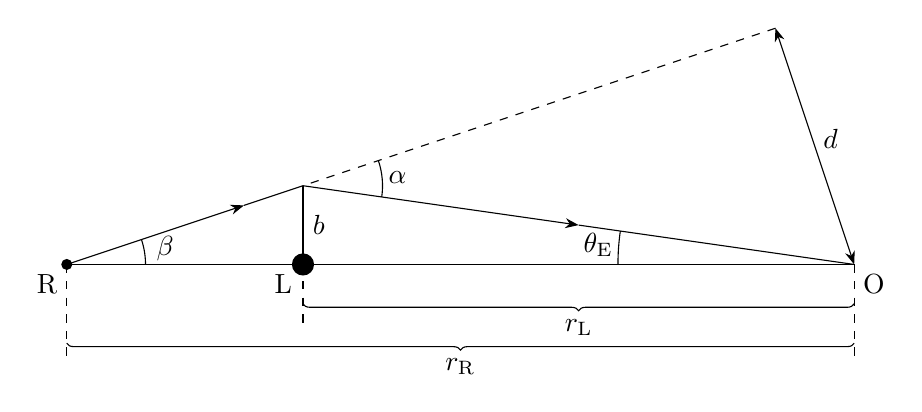
\begin{tikzpicture}[>=Stealth]
                \draw [->] (0,0) -- (2.25,0.75);
                \draw (2.25,0.75) -- (3,1);
                \draw [dashed] (9,3) -- (3,1);
                \draw (0,0) -- (10,0);
                \draw [->] (3,1) -- (6.5,0.5);
                \draw (6.5,0.5) -- (10,0);
                \fill (0,0) circle [radius=2pt];
                \fill (3,0) circle [radius=4pt];
                \draw (2.75,-0.25) node {L};
                \draw (10.25,-0.25) node {O};
                \draw (-0.25,-0.25) node {R};
                \draw (7,0) arc [start angle=180,radius=3,delta angle=-8.13010];
                \draw (1,0) arc [start angle=0,radius=1,delta angle=18.43495];
                \draw (4,0.85714) arc [start angle=-8.13010,radius=1,delta angle=26.56505];
                \draw (6.75,0.25) node {$\theta_{\mathrm{E}}$};
                \draw (4.2,1.1) node {$\alpha$};
                \draw (1.25,0.2) node {$\beta$};
                \draw (3,0) -- (3,1);
                \draw [<->] (10,0) -- (9,3);
                \draw (3.2,0.5) node {$b$};
                \draw (9.7,1.6) node {$d$};
                \draw [decorate,decoration=brace] (10,-1) -- (0,-1);
                \draw (5,-1.3) node {$r_\mathrm{R}$};
                \draw [decorate,decoration=brace] (10,-0.5) -- (3,-0.5);
                \draw (6.5,-0.8) node {$r_\mathrm{L}$};
                \draw [dashed] (0,0) -- (0,-1.25);
                \draw [dashed] (10,0) -- (10,-1.25);
                \draw [dashed] (3,0) -- (3,-0.75);
            \end{tikzpicture}
        \end{center}
        
        由几何关系及光线在引力透镜下的偏折角$\alpha = \dfrac{4GM_0}{bc^2} = \dfrac{4M}{b}$可得：
        \begin{equation}
            \theta_{\mathrm{E}} = \frac{b}{r_{\mathrm{L}}}
        \end{equation}
        \begin{equation}
            \alpha = \frac{d}{r_{\mathrm{L}}} = \frac{4M}{b}
        \end{equation}
        \begin{equation}
            \beta = \frac{b}{r_{\mathrm{R}} - r_{\mathrm{L}}} = \frac{d}{r_{\mathrm{R}}}
        \end{equation}
        这里使用了小角近似：$\theta \ll 1$时，有$\sin\theta = \tan\theta = \theta$。
        
        联立(2)、(3)两式得：
        \[
        d = \frac{b r_{\mathrm{R}}}{r_{\mathrm{R}} - r_{\mathrm{L}}}
        \]
        代入(2)得：
        \[
        \frac{4M}{b} = \frac{b r_{\mathrm{R}}}{(r_{\mathrm{R}} - r_{\mathrm{L}})r_{\mathrm{L}}}
        \]
        即：
        \[
        b = \sqrt{\frac{4M(r_{\mathrm{R}} - r_{\mathrm{L}})r_{\mathrm{L}}}{r_{\mathrm{R}}}}
        \]
        则Einstein环的半径为：
        \[
        \theta_{\mathrm{E}} = \frac{b}{r_{\mathrm{L}}} = \sqrt{\frac{4M(r_{\mathrm{R}} - r_{\mathrm{L}})}{r_{\mathrm{R}} r_{\mathrm{L}}}}
        \]

    \end{itemize}

\end{document}